%% Copernicus Publications Manuscript Preparation Template for LaTeX Submissions
%% ---------------------------------
%% This template should be used for copernicus.cls
%% The class file and some style files are bundled in the Copernicus Latex Package, which can be downloaded from the different journal webpages.
%% For further assistance please contact Copernicus Publications at: production@copernicus.org
%% https://publications.copernicus.org/for_authors/manuscript_preparation.html


%% Please use the following documentclass and journal abbreviations for preprints and final revised papers.

%% 2-column papers and preprints
\documentclass[journal abbreviation, manuscript]{copernicus}



%% Journal abbreviations (please use the same for preprints and final revised papers)


% Advances in Geosciences (adgeo)
% Advances in Radio Science (ars)
% Advances in Science and Research (asr)
% Advances in Statistical Climatology, Meteorology and Oceanography (ascmo)
% Aerosol Research (ar)
% Annales Geophysicae (angeo)
% Archives Animal Breeding (aab)
% Atmospheric Chemistry and Physics (acp)
% Atmospheric Measurement Techniques (amt)
% Biogeosciences (bg)
% Climate of the Past (cp)
% DEUQUA Special Publications (deuquasp)
% Earth Surface Dynamics (esurf)
% Earth System Dynamics (esd)
% Earth System Science Data (essd)
% E&G Quaternary Science Journal (egqsj)
% EGUsphere (egusphere) | This is only for EGUsphere preprints submitted without relation to an EGU journal.
% European Journal of Mineralogy (ejm)
% Fossil Record (fr)
% Geochronology (gchron)
% Geographica Helvetica (gh)
% Geoscience Communication (gc)
% Geoscientific Instrumentation, Methods and Data Systems (gi)
% Geoscientific Model Development (gmd)
% History of Geo- and Space Sciences (hgss)
% Hydrology and Earth System Sciences (hess)
% Journal of Bone and Joint Infection (jbji)
% Journal of Micropalaeontology (jm)
% Journal of Sensors and Sensor Systems (jsss)
% Magnetic Resonance (mr)
% Mechanical Sciences (ms)
% Natural Hazards and Earth System Sciences (nhess)
% Nonlinear Processes in Geophysics (npg)
% Ocean Science (os)
% Polarforschung - Journal of the German Society for Polar Research (polf)
% Primate Biology (pb)
% Proceedings of the International Association of Hydrological Sciences (piahs)
% Safety of Nuclear Waste Disposal (sand)
% Scientific Drilling (sd)
% SOIL (soil)
% Solid Earth (se)
% State of the Planet (sp)
% The Cryosphere (tc)
% Weather and Climate Dynamics (wcd)
% Web Ecology (we)
% Wind Energy Science (wes)


%% \usepackage commands included in the copernicus.cls:
%\usepackage[german, english]{babel}
%\usepackage{tabularx}
%\usepackage{cancel}
%\usepackage{multirow}
%\usepackage{supertabular}
%\usepackage{algorithmic}
%\usepackage{algorithm}
%\usepackage{amsthm}
%\usepackage{float}
%\usepackage{subfig}
%\usepackage{rotating}

\usepackage{booktabs} 
\usepackage{adjustbox}
\usepackage{longtable}

\begin{document}

\title{Urban Ozone Trends in Europe and the USA (2000-2021)}

% \Author[affil]{given_name}{surname}

\Author[1,2,*][beth.nelson@york.ac.uk]{Beth S.}{Nelson} %% correspondence author
\Author[1,2,*][will.drysdale@york.ac.uk]{Will S.}{Drysdale}

\affil[1]{Wolfson Atmospheric Chemistry Laboratories, Department of Chemistry, University of York, Heslington, York, YO10 5DD, UK}
\affil[2]{National Centre for Atmospheric Science, University of York, York, UK}
\affil[*]{These authors contributed equally to this work.}
%% The [] brackets identify the author with the corresponding affiliation. 1, 2, 3, etc. should be inserted.

%% If an author is deceased, please mark the respective author name(s) with a dagger, e.g. "\Author[2,$\dag$]{Anton}{Smith}", and add a further "\affil[$\dag$]{deceased, 1 July 2019}".

%% If authors contributed equally, please mark the respective author names with an asterisk, e.g. "\Author[2,*]{Anton}{Smith}" and "\Author[3,*]{Bradley}{Miller}" and add a further affiliation: "\affil[*]{These authors contributed equally to this work.}".


\runningtitle{TEXT}

\runningauthor{TEXT}

\received{}
\pubdiscuss{} %% only important for two-stage journals
\revised{}
\accepted{}
\published{}

%% These dates will be inserted by Copernicus Publications during the typesetting process.


\firstpage{1}

\maketitle


\begin{abstract}
No abstract yet.
%Trends in urban O\textsubscript{3} and NO\textsubscript{2} across Europe and the United States of America were explored between 2000-2021. Using surface monitoring site data from the TOAR-II and European Environment Agency databases, piecewise quantile regression (PQR) analysis was performed on 228 O\textsubscript{3} time series (144 European, 84 USA) and 322 NO\textsubscript{2} times series (245 European, 77 USA). The PQR analysis permitted 2 break points over the 23 year period to balance the intent to describe changes over a large time period, while still capturing the abrupt changes that can occur in urban atmospheres. Regressions were performed over quantiles ranging from 0.05 to 0.95 and indications of a slowing in the increase of high European O\textsubscript{3} levels was observed. In Europe, more trends were found to having an increasing O\textsubscript{3} trend between 2015-2021 compared with 2000-2004. The reverse was true in the USA, with a reduction in the number of sites with increasing O\textsubscript{3} trends when the same periods were compared. An analysis of the change points revealed a large proportion of sites in Europe, were the second change point in NO\textsubscript{2} switched from a positive to negative trend, occurred in 2020 (41/43 second change points in this year). This was attributed a reduction in NO\textsubscript{2} due to the COVID-19 pandemic, however, in some cases these increasing trends have sustained beyond the recovery from restrictions. 
\end{abstract}

\section{Introduction}  %% \introduction[modified heading if necessary]
Tropospheric ozone (O\textsubscript{3}) is a greenhouse gas and air pollutant harmful to human health, and plant growth \citep{fleming_2018, mills_2018, szopa_2021}. It is a secondary air pollutant, formed from the photochemical reactions of primary pollutants NO\textsubscript{x} (NO + NO\textsubscript{2}) and volatile organic compounds (VOCs). The chemistry of O\textsubscript{3} formation is non-linear and the effect of changing precursor concentrations can cause O\textsubscript{3} concentrations to increase or decrease depending on the photochemical regime found at a given location \citep{ https://doi.org/10.1029/JD095iD02p01837, SILLMAN2002339}. Despite global successes in reducing primary pollutant emissions over the past few decades, global exposure to O\textsubscript{3} has been increasing throughout the 21st century. This is particularly observed in urban areas, where the vast majority of the global population live, projected to increase to 68\% in 2050 from 55\% in 2018 \citep{un_2019}. In a study of 12946 cities located worldwide, the average mean weighted O\textsubscript{3} concentration increased by 11\% between 2000 and 2019, and the number of cities exceeding the WHO peak season O\textsubscript{3} standard increased from 89\% to 96\% \citep{Malashock_2022}.

Due to the complexity of O\textsubscript{3} production, its trend direction, magnitude, and significance varies by location. The Tropospheric Ozone Assessment Report Phase I (TOAR I) was the first global review of trends in surface ozone, covering 1970 - 2014 \citep{fleming_2018, Gaudel2018}. As part of the TOAR-I review, trends in two O\textsubscript{3} metrics were calculated globally over the period of 2000 - 2014: 4th highest daily maximum 8-hour O\textsubscript{3} (4MDA8), and the number of days with MDA8 > 70 ppb O\textsubscript{3} (NDGT70) \citep{fleming_2018}. The study used data from 4801 global monitoring sites over this time period. For both of these metrics, downward trends were observed for most of the USA, and some sites in Europe. However, over the period of 2010-2014 (2,600 sites utilised), sites located in regions with the highest O\textsubscript{3} precursor emissions across North America, Europe and East Asia had the highest values in 4MDA8 and NDGT70. In North America and Europe, this was particularly true for California and parts of Southern Europe \citep{fleming_2018}.

Since the 1990s, a general downward trend in urban O\textsubscript{3} pollution has been observed in the United States \citep{acp-20-3191-2020}. This reducing trend has been linked to stricter limiting regulations on the emissions of primary pollutants such as NO\textsubscript{x} and VOCs. Although NO\textsubscript{x} and VOC emissions in Europe have also been declining since the late 1980s, the trend in O\textsubscript{3} is less clear due to large inner-annual variation, driven by climate variability and the dispersion and transport of pollutants from other regions \citep{acp-6-51-2006, acp-18-5589-2018}. Between 1995 and 2014, negative trends in the highest O\textsubscript{3} levels across urban sites in Europe were identified due to pollutant emission restrictions across Europe. However, increasing background levels, particularly in northern and eastern Europe, make it difficult to identify strong trends in urban O\textsubscript{3} when transboundary effects are considered \citep{acp-18-5589-2018}. Despite this, a study of 93 suburban and urban sites across Europe identified notable enhancements in O\textsubscript{3} seasonal and annual means between 1995 - 2012, even with the continuous downward trend in anthropogenic emissions across the continent \citep{acp-18-5589-2018}.

%Since these earlier studies, much of the literature focuses on the impact of the COVID-19 pandemic on air pollutant concentrations and trends \citep{acp-20-15743-2020, doi:10.1126/sciadv.abd6696, acp-21-4169-2021, SOKHI2021106818}. A study of eleven cities across the world, all of which implemented stringent lockdown measures in early 2020, captured sudden decreases in deweathered NO\textsubscript{2} concentrations, concurrent with sudden increases in O\textsubscript{3}, in most locations \citep{doi:10.1126/sciadv.abd6696}. Another study employing machine learning models to predict business-as-usual levels of pollutants, estimated that NO\textsubscript{2} concentrations were 32\% lower than expected across 102 European urban background locations, whereas O\textsubscript{3} was 21\% higher \citep{acp-21-4169-2021}. It is highly likely that this global event has resulted in perturbations of both long-term NO\textsubscript{2} and O\textsubscript{3} trends, particularly in locations where lockdowns were stringent or lengthy.

In this study, we aim to expand of the work of \cite{fleming_2018}, to investigate a longer time-series of 21st century trends (2000 - 2021). Here, we focus on the trends in urban O\textsubscript{3}, complimented by NO\textsubscript{2} timeseries data, using urban monitoring site data from Europe and the United States of America across the 21 year period. We employ quantile regression and change point detection to construct trends that capture the broad structure of a complex time series, while remaining explainable with concise statistics. To gain a clearer understanding of the group behaviour of sites, we use hierarchical clustering (HC) with dynamic time warping (DTW), recently developed by REF, to group together 21 year time series with comparable time-series structures within Europe and the United States of America independently. This is then used to investigate whether trends in MDA8, and both episodic and exposure-relevant O$_3$ metrics, are varying regionally. Our analysis focuses comparisons between warm-season and cold-season MDA8 values, as well as probing different changes across quantiles, to allow for an assessment of whether low or high O$_3$ distributions have different behaviours, across Europe and the USA, and between hierarchical clusters.

\section{Methodology} \label{sect:method}

\subsection{Data Preparation} \label{sect:data_prep}
Hourly NO\textsubscript{2} and O\textsubscript{3} data were obtained for urban sites in the USA and Europe using the TOAR-II \citep{toar_db} and European Environment Agency (EEA) \citep{eea_1, eea_2} databases, using the r-packages \emph{toarR} \citep{drysdale_2024_14537446} and \emph{saqgetr} \citep{saqgetr} respectively. Those obtained from the EEA are categorised as urban traffic, urban background and urban industrial, while those from the TOAR database are categorised as urban and suburban. A full list of sites can be found in the supplementary information (table S1).  TOAR-II data was retrieved between 2000-01-01 and 2021-12-31 (the latest available) \textcolor{red}{and EEA data between 2000-01-01 and 2023-12-31, the latter being extended longer so the effects of the COVID-19 pandemic could be observed more clearly.} Time series were quality controlled via threshold, persistence and variance checks similar to those in \textcolor{red}{Wang et al., 2024 - or reference within}: O\textsubscript{3} concentrations were required be between 0 and 500 ppbv, periods where an identical value was repeated 8 or more times in a row were removed as were days where the difference between the minimum and maximum concentration was $\leq$ 2 ppbv. 

After quality control, time series were required to have 80 \% data coverage between 2000-01-01 and 2021-12-31 and for the calculation of annual metrics each individual year was retained if it had more than 60 \% coverage. Additionally, a small number of time series were removed following visual inspection - these are listed in table \textcolor{red}{S2}. This resulted in 360 O\textsubscript{3} time series (208 Europe, 152 USA). Trends were calculated on daily averaged data, either the mean or maximum daily 8-hour average (MDA8). 

For the mean data, subgroups of day (hours between 0800 - 1900 L inclusive) and night (hours between 2000 - 0700 L inclusive) were created, and for both mean and MDA8 data subgroups of warm (April - September) and cold (October - March) season were created (table \ref{tab:ts_types}). It is common to remove the seasonal component of an ozone time series to improve the accuracy of trends \citep{cooper_2020} and here we subtract monthly mean climatologies for each time series resulting ozone anomalies. 

\begin{table}[h]
\caption{Types of time series for which trends have been calculated \textcolor{red}{Could go in SI}}
\begin{tabular}{c|c c c}
Type              & Averaging & Hours         & Months            \\ \hline
Daily             & mean      & All           & All               \\
Daily Day         & mean      & 0800 - 1900 L & All               \\
Daily Day Warm    & mean      & 0800 - 1900 L & April - September \\
Daily Day Cold    & mean      & 0800 - 1900 L & October - March   \\
Daily Night       & mean      & 2000 - 0700 L & All               \\
Daily Night Warm  & mean      & 2000 - 0700 L & April - September \\
Daily Night Cold  & mean      & 2000 - 0700 L & October - March   \\
MDA8              & MDA8      & All           & All               \\
MDA8 Warm         & MDA8      & All           & April - September \\
MDA8 Cold         & MDA8      & All           & October - March   \\
\end{tabular}
\label{tab:ts_types}
\end{table}

\subsection{Metrics}

\subsection{Trend Analysis}
Trends were estimated for these daily, daily day, daily night and MDA8 series in three cases: all data, warm season (April - September) and cold season (October - March). These were calculated following the methodology in and using code provided by  \cite{chang2023guidancenotebeststatistical}. QR calculates a linear model that seeks to minimise the residuals with a defined proportion ($\tau$) of the points above and below the fit line. For example, the scenario $\tau$ = 0.5 splits the data 50:50 above and below the line. QR has the advantage of being insensitive to outliers and the $\tau$ = 0.5 case can be considered analogous to a “median” trend line. This is desirable for the longer-term trends being investigated here. The 1-sigma uncertainly for the QRs were calculated via a moving block bootstrapping method, where the data are subdivided into overlapping blocks that are $n^{1/4}$ points wide (or \textasciitilde{20} points for 20 years of hourly data). These blocks are shuffled to generate a new time series, and replicated 1000 times, and the standard deviation of these replicates calculated. This uncertainty was subsequently used in the determination of the p-value, providing a metric for the significance of the trends. 

Quantile regressions were calculated piecewise with 0 - 2 breakpoints to allow the trends to capture large non-linearities. As urban concentration trends can change sharply (e.g. with policy intervention), this gives the model the freedom to represent these. Limiting the model to a maximum of two breakpoints strikes a balance between capturing sufficiently large-scale changes while still being able to describe a \textasciitilde{20} year time series with a small number of coefficients.

To determine what break points to use on each time series, a range of candidate models were constructed, each with zero, one or two break points. These break points were restricted to be unable to occur within the first or last two years of the time series, nor could they occur within 5 years of each other. They were arbitrarily set to occur on the 1st January in a given year, which was deemed an appropriate degree of freedom given the 20 year span of the time series and locating the break points sub annually does not have a large effect on the resulting trends. For a time series that fully spanned the range of 2000-01-01 - 2021-12-31, 110 models would be created - one with zero break points, 18 with one break point, and 91 with 2. All regressions were calculated at $\tau$ = 0.05, 0.10, 0.25, 0.50, 0.75, 0.95 and 0.95.

To select 'change points' from the array of break points available, the model performance was evaluated via Akaike information criterion (AIC). AIC was chosen as the evaluation criteria oweing to its penalty term penalising models with more break points that do not appreciably improve the model fit over the simpler case, The model with the minimum AIC was selected from the candidate pool as the best fit for a time series at a given $\tau$. 

Trends have been collated into significance categories: p $\le$ 0.05 (high certainty), 0.05 $<$ p $\le$ 0.10 (medium certainty), 0.10 $<$ p $\le$ 0.33 (low certainty) and p > 0.33 (very low certainty or no evidence) based off of the guidance of \cite{chang2023guidancenotebeststatistical}. For the most part slopes where the p-value is > 0.33 are treated as ‘no trend’ regardless of their magnitude (generally we observe that as the magnitude of the trend decreases so does its significance), though sometimes are given with a direction when required by a visualisation.

\subsection{Clustering} \label{sect:method_clustering}
To aid analysis it was desirable to group similar time series, clusters were calculated using hierarchical clustering (HC) with dynamic time warping (DTW) used as a distance measure \citep{AGHABOZORGI201516}. DTW provides a distance measure between two time series that allows for some deviation in the relation of features in time and one-to-many mapping of features, as opposed to use of e.g. the euclidean distance where mapping between series is one-to-one and cannot undergo deformation \citep{Berndt_dtw, Abdullah_Keogh_dtw}. We adopt a similar method to \cite{REED2025110686} using the R package \emph{dtwclust} \citep{dtwclust} for both DTW and HC steps, and used to calculate cluster validity indices (CVIs). Clustering was performed by region and time series type (e.g sites in Europe for the MDA8-O3 warm season). Time series were normalised and then, to provide clusters related to the range of $\tau$ values used in the QRs, aggregated monthly by calculating the $\tau^{th}$ quantile per month. Metrics were not aggregated as they are all annual values. Clustering was calculated with 5 - 75 clusters, and then evaluated with 6 internal CVIs (Silhouette, Dunn, Calinski-Harabasz, COP, Davies-Bouldin and Modified Davies-Bouldin) where the latter 3 were inverted such that all can be maximised. The final selection for the number of clusters was determined as the mean of the optimal number of clusters suggested by each of the CVIs. 

\clearpage
\section{Results and Discussion}

\begin{figure*}[t]
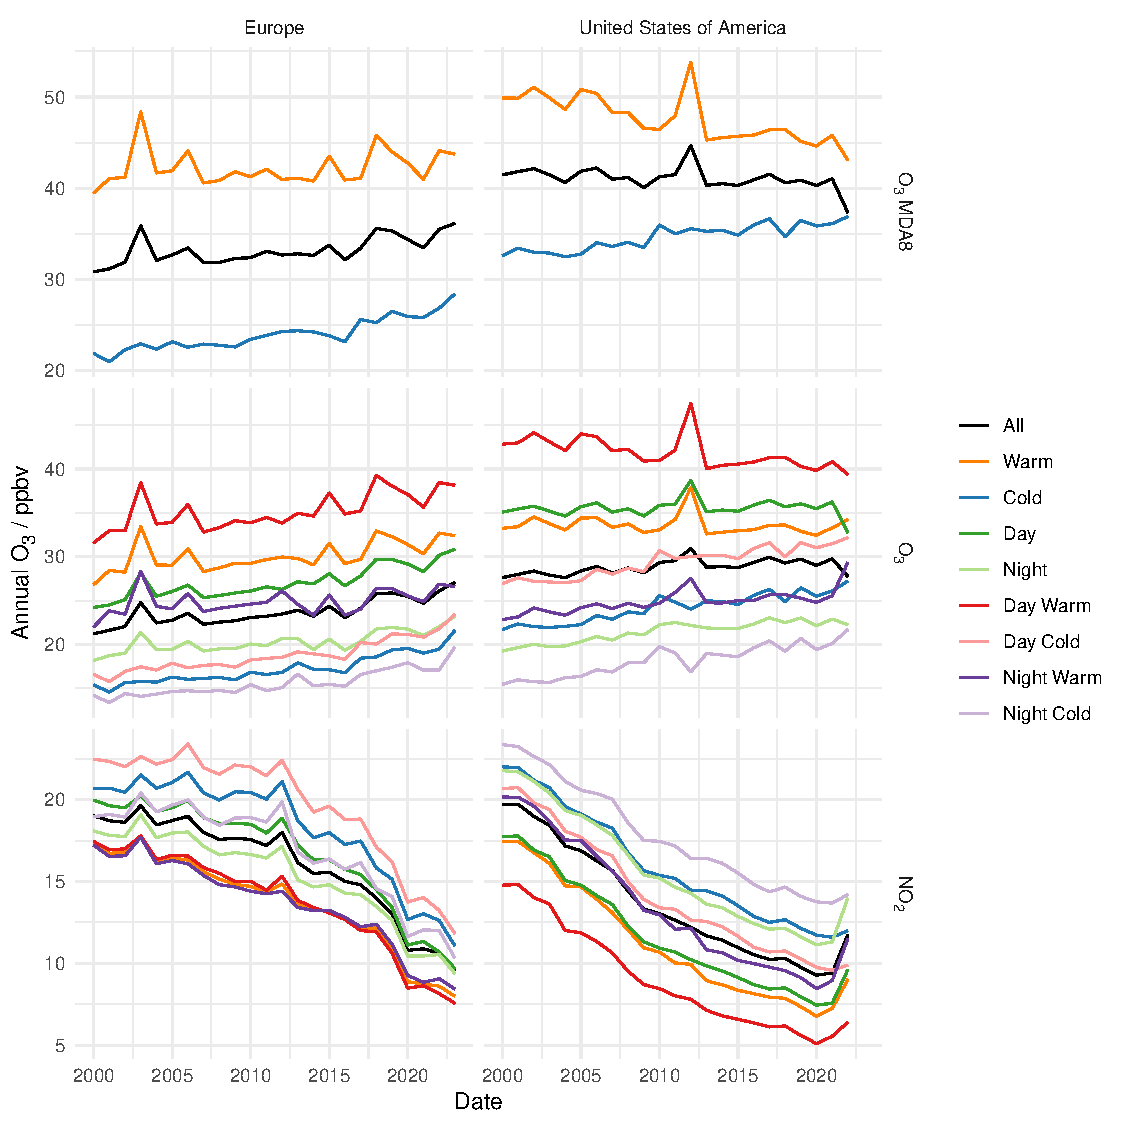
\includegraphics[width=12cm]{figures/paper_figures/f2.pdf}
\caption{Time series of annual average MDA8O\textsubscript{3}, O\textsubscript{3} and NO\textsubscript{2} for urban sites in Europe and the USA, for the time series types detailed in (table \ref{tab:ts_types})}
\label{fig:conc_plot}
\end{figure*}

As an initial overview, figure \ref{fig:conc_plot} shows the annual mean concentrations across the range of all the urban sites and time series types used in the this study (table \ref{tab:ts_types}). European O\textsubscript{3} concentrations show a steady increase over the last 20 years, with the average across all data increasing from 21.2 ppbv in 2000 to 25.9 ppbv in 2019, the MDA8O\textsubscript{3} increasing from 30.8 to 35.3 ppbv and warm season MDA8O\textsubscript{3}. In the USA average O\textsubscript{3} has increased from 27.7 to 29.7 ppbv, but MDAO\textsubscript{3} and warm season MDA8O\textsubscript{3} both decreased, from 41.5 to 40.9 and 49.9 to 45.1 ppbv respectively. Annual average urban NO\textsubscript{2} is also shown to provide some context to precursor concentrations. Both Europe and the USA have seen reductions in NO\textsubscript{2}, 19.0 in 2000 to 13.0 ppbv in 2019 in Europe and 19.7 to 9.8 ppbv in the USA. The USA did see a minima in 2020 of 9.3 ppbv, but increased to 11.8 ppbv in 2022, whereas Europe continued its decrease to 10.6 ppbv in 2022. 

The other features that do stand out appear in the sub groups containing the warm season, but are most clear in the warm MDA8O\textsubscript{3} series correspond to years with significant heatwaves - 2003, 2006, 2015 and 2018 in Europe and 2012 in the USA. Heat waves are historically linked to enhanced O\textsubscript{3} concentrations, and are expected to increase in frequency \citep{Schär2004, Russo_2015, https://doi.org/10.1002/2016GL068432, Otero_2016, GOULDSBROUGH2022118975}. The continued impact of heat waves on high O\textsubscript{3} is however, dependant on the future levels of O\textsubscript{3} precursors and reductions and indeed this can be observed at some sites \citep{Meehl_2018, OTERO2021118334, acp-25-2725-2025, acp-25-5101-2025}, but urban sites may take longer to reach levels where O\textsubscript{3} - temperature sensitivity is reduced, owing to a higher initial concentrations \citep{VazquezSantiago2024}.


\subsection{Change Point Assignment} \label{sect:new_mda8_piecewise_types}

Regional differences were observed in the types (QR, PQR\_1, PQR\_2) of change point assigned. Figure \ref{fig:regression_type} shows that O\textsubscript{3} series (daily mean, MDA8O\textsubscript{3} and MDA8O\textsubscript{3} warm season, across all values of $\tau$) in Europe were rarely described by QR (1 - 3 \% of series), whereas the United States of America was described by it 30 - 62 \% of the time. A similar trend is seen across all types of time series (\textcolor{red}{SI}). As the European time series extend to 2023, some of these additional change points are likely due to the COVID pandemic, and indeed examining the location of change points by year (\textcolor{red}{SI}) shows an increased number of change points in 2019 - 2021 in Europe - this is also reflected in the (fewer) change points seen in the USA. This also highlights that there are more change points focused at the beginning and end of the series generally (for both O\textsubscript{3} and NO\textsubscript{2}) which may indicate some edge effects from the selection process. However, we don't expect this to have impacted our results as the method demonstrates the ability to choose regressions with zero change points, we do not observe large swings in trends overall at these times (\textcolor{red}{reference slopes/significance bars section}) and that there is a good amount of other change points assigned within the time period.
 
\begin{figure}[h!]
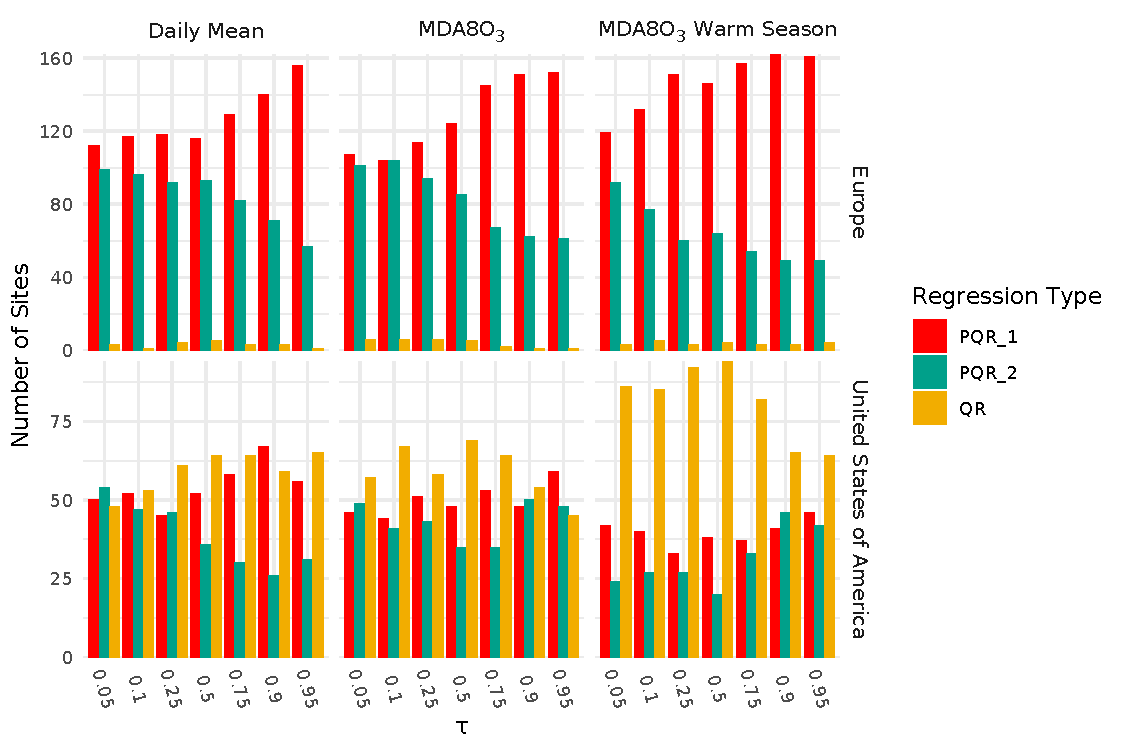
\includegraphics[width=12cm]{figures/paper_figures/regression_type_bars_o3.pdf}
\caption{Number of sites with no change point (QR, gold), one change point (PQR\_1, red) and two change points (PQR\_2, green) in the Daily Mean, MDA8O\textsubscript{3} and MDA8O\textsubscript{3} warm season series, separated into Europe and United States of America regions.}
\label{fig:regression_type}
\end{figure}



%%%%%%%%%%%%%%%%%%%%%%%%%%%%%%%%%%%%%%%%%%%%%%%%%%%%

\subsection{Trends in MDA8 Across Quantiles} \label{sect:new_mda8_trends}

Trends in MDA8 for each site at a range of different quantiles were calculated using the methodology described in section \ref{sect:method_clustering}. Figure \ref{fig:p_bar_year_mda8_anom_combined} shows the number of sites with increasing and decreasing trends for a selection of quantiles (5\textsuperscript{th}, 50\textsuperscript{th} and 95\textsuperscript{th}), for each year between 2004 and 2018, as well as the degree of certainty of the trends, in the MDA8 O$_3$ data. Generally, there are a large proportion of high certainty positive trends in the 5\textsuperscript{th} and 50\textsuperscript{th} percentile in the EU data set (range of 34 - 72\% of trends across the 20-year period). In contrast there are fewer trends of high certainty in the 95\textsuperscript{th}, the majority of which are decreasing (between 5 - 25\% across the 20-year period). The warm-season data shows a similar pattern, but with fewer high certainty increasing trends in the 5\textsuperscript{th} and 95\textsuperscript{th} percentile. Many more high certainty increasing trends are observed in the cold season only data, particularly in the 5\textsuperscript{th} and 50\textsuperscript{th} percentile data (range of 29 - 73\% across the 20-year period). The proportion of high certainty increasing trends in the cold season appears to be increasing with time.

In the US MDA8 trend data, the majority of 5\textsuperscript{th} percentile trends are high certainty increasing trends (35 - 53\%) and the 95\textsuperscript{th} percentile is dominated by high certainty negative trends (46 - 76\%), with a mixture found in the 50\textsuperscript{th} percentile. This is consistent with the findings of \cite{Simon_2015} who observed increasing O3 trends across urban sites in the US (1998 - 2013) at the lower end of the O$_3$ distribution, and decreasing trends at the upper end, leading to an observed compression of the O$_3$ range. In the warm-season only data, there is a larger contribution of decreasing trends across all percentiles. This is particularly true in the 95\textsuperscript{th} percentile data, where the vast majority of trends are high certainty decreasing trends (55 - 84\%). However, there is a notable change year-on-year in the US 95\textsuperscript{th} warm-season dataset that is worth some discussion. Although decreasing trends dominate, and the number of high certainty increasing trends are low (1-11\%), we observed a step-change. Between 2000 - 2008, between 1-3\% of trends are high certainty increasing trends. However, after 2008, the number of sites showing a high certainty increasing trend increases rapidly from 2 to 16 by 2016, with the majority of these sites located in Western and Central US, and the top three largest magnitude slopes (medium-large), located in the South. In the cold season data, there is very little year-on-year change in the distribution of increasing and decreasing trends in the 5\textsuperscript{th}, 50\textsuperscript{th} and 95\textsuperscript{th} percentile. high certainty.
% Do we want to talk about these sites? Regionality?

\begin{figure}[h!]
\centering
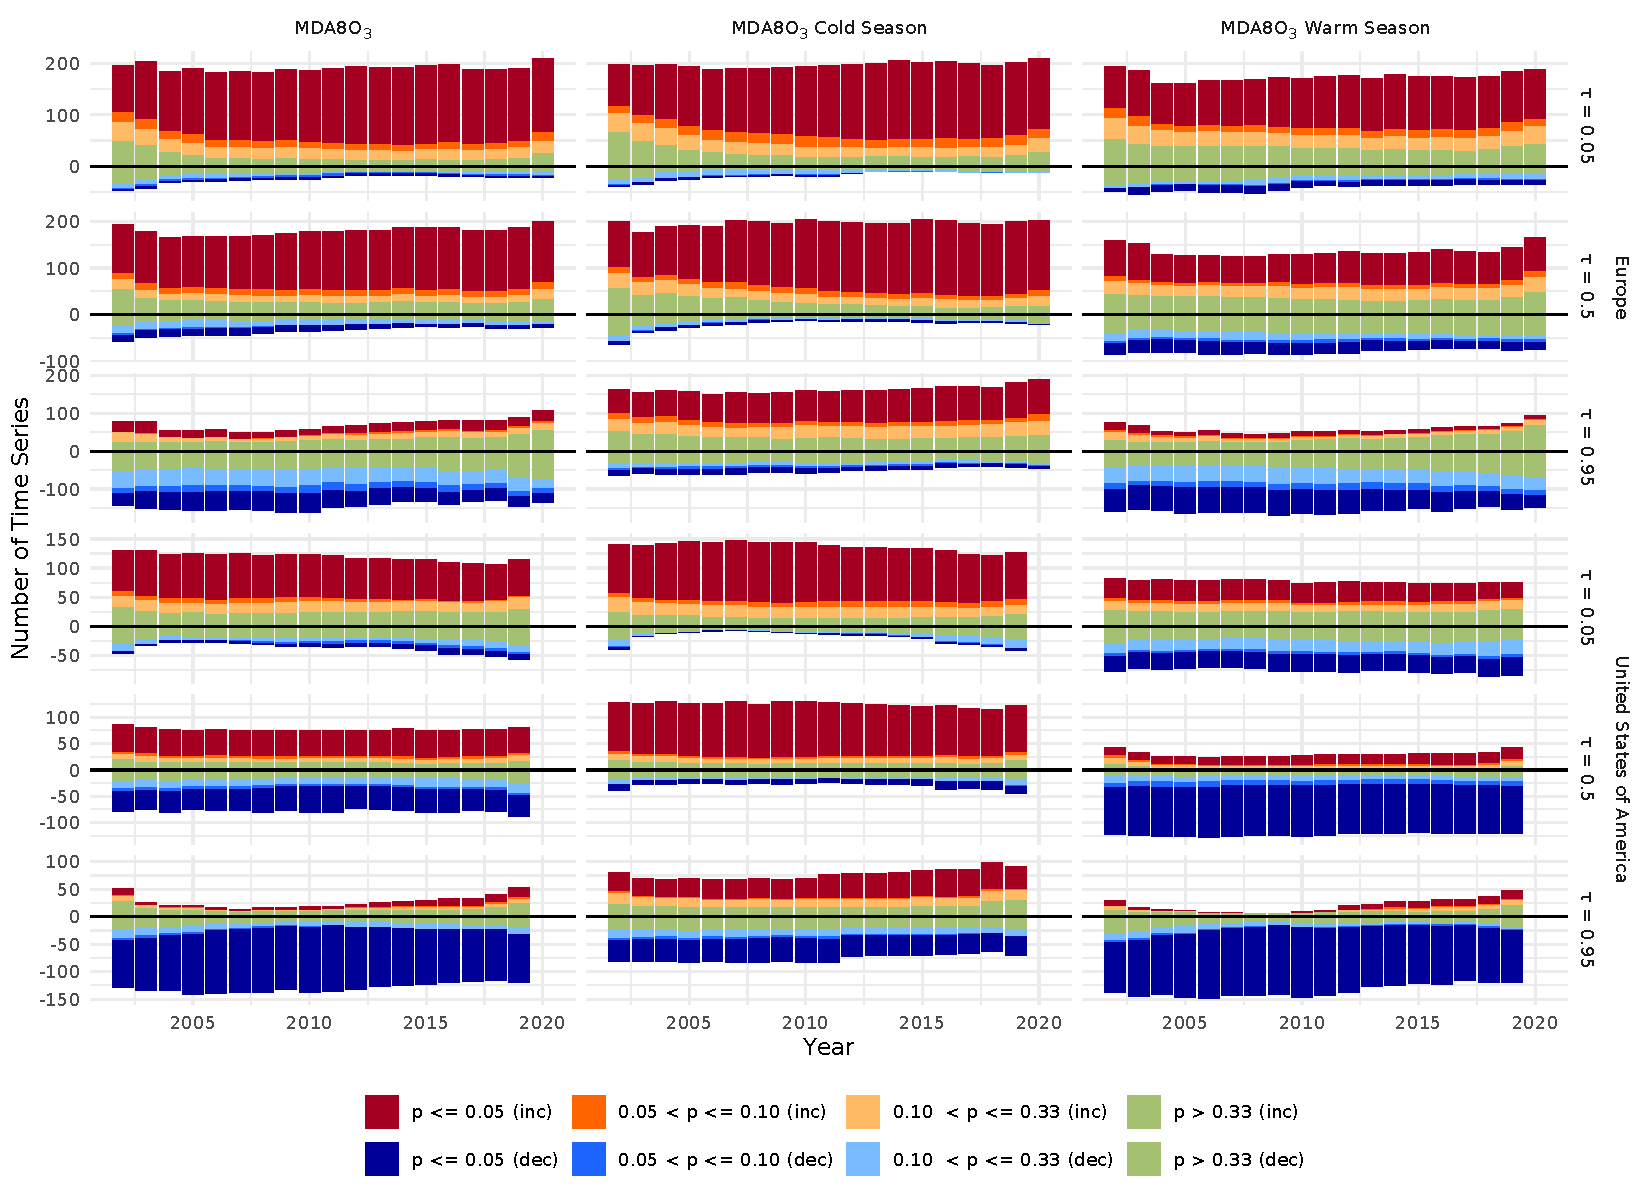
\includegraphics[width=\textwidth]{figures/paper_figures/signifcance_bars.pdf}
\caption{Time series of trends in MDA8 O\textsubscript{3} for (left) annual, (middle) warm season, and (right) cold season, for Europe (top) and the USA (bottom). Within each region the panels are grouped by $\tau$ = 0.05 (top), 0.5 (middle), 0.95 (bottom)}
\label{fig:p_bar_year_mda8_anom_combined}
\end{figure}

The distribution of slopes and the corresponding uncertainty of each trend is shown in Figure XXX for the 5\textsuperscript{th}, 50\textsuperscript{th} and 95\textsuperscript{th} quantiles and for one year near the beginning (2004), and one near the end (2018) of the 21-year time period (additional quantiles and years are found in the supplementary), and an overview of the trend distributions is presented here. We use p-values to describe the certainty of each trend, as defined by \cite{chang2023guidancenotebeststatistical}. The magnitude of each trend is prescribed as "small", "medium", large" or "very large", according to the ranges described in Table \ref{tab:magnitude_description_table}.

\begin{figure}[h!]
\centering
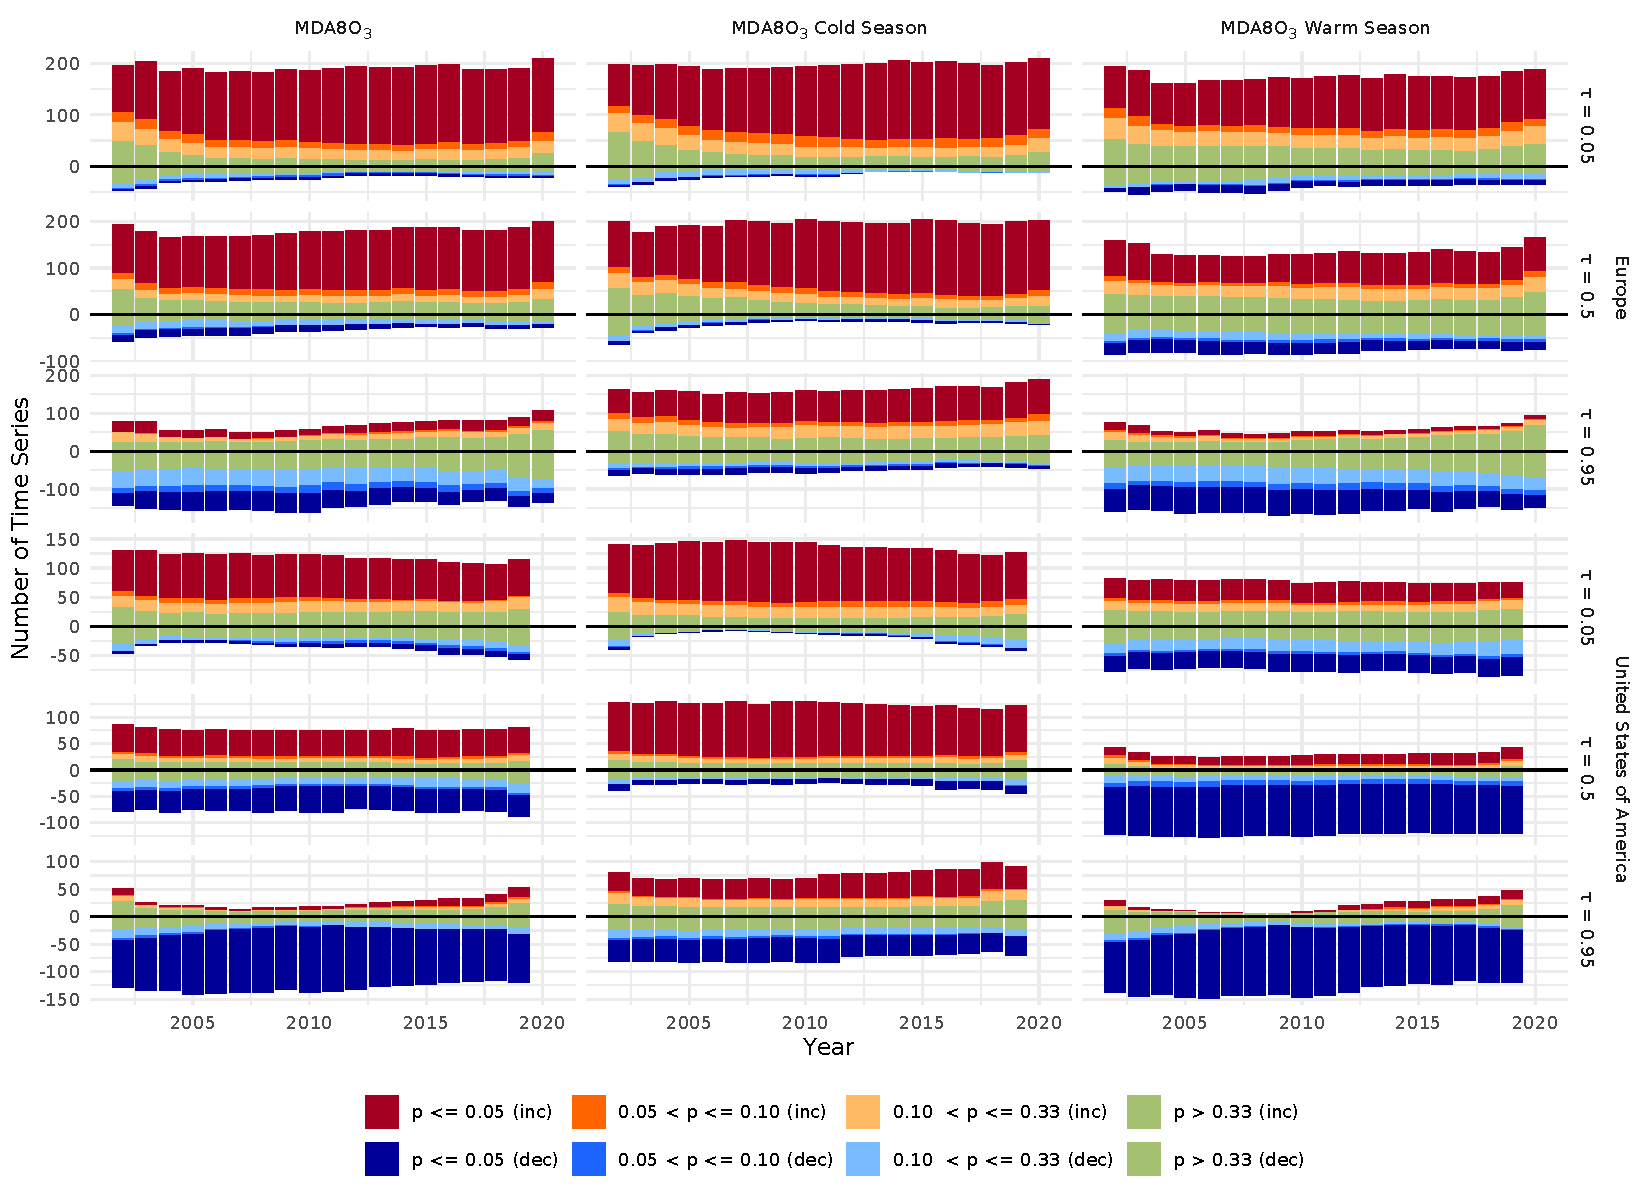
\includegraphics[width=\textwidth]{figures/paper_figures/signifcance_bars.pdf}
\caption{}
\label{fig:o3_map_eu_mda8}
\end{figure}


\begin{table}[h]
\caption{Description of trend magnitude ranges.}
\begin{tabular}{c|c}
Range / ppb yr$^{-1}$                 & Magnitude description \\ \hline
0 \textless slope \textless 0.5       & small                 \\
0.5 \textless{}= slope \textless 1.5  & medium              \\
1.5 \textless{}= slopes \textless 2.5 & large                 \\
slope \textgreater{}= 2.5             & very large           
\end{tabular}
\label{tab:magnitude_description_table}
\end{table}

Across the EU data set at the start of the century (2004), 85\% and 78\% of slopes showed an increasing trend in the 5\textsuperscript{th} and 50\textsuperscript{th} quantiles respectively (73\% and 57\% of total at moderate certainty or higher respectively), compared to 74\% showing a decreasing trend in the 95\% quantile (31\% of total at moderate certainty or higher). By 2018, the number of increasing slopes increased across the three quantiles, to 90\% and 86\% for the 5\textsuperscript{th} and 50\textsuperscript{th} quantile (74\% and 69\% of total at moderate certainty or higher), and from 26\% to 39\% in the 95\textsuperscript{th} quantile (from 7\% to 15\% of total at moderate certainty or higher). This supports an increase in the number of EU sites with increasing O$_3$ trends at the end of the two-decadal period compared to the beginning, for which the majority of sites showed increasing trends in the low-mid quantiles during both time periods. In the 95\textsuperscript{th} quantile, the majority of sites were are showing decreasing trends in both time periods, but a larger proportion of increasing trends is apparent in 2018 compared to 2004. 

In comparison, 82\%  and 49\% of slopes showed an increasing trend in the 5\textsuperscript{th} and 50\textsuperscript{th} quantiles of the US data set at the start of the century (56\% and 36\% of total at moderate certainty or higher). Similarly to the EU, 95\textsuperscript{th} quantile trends were decreasing the in US (87\% - 68\% of total at moderate certainty or higher). However, in contrast to EU, by 2018 fewer trends were increasing, down to 68\% in the 5\textsuperscript{th} quantile (40\% of total at moderate certainty or higher), from 82\% in 2004 (56\% of total at moderate certainty or higher). In the 50\textsuperscript{th} quantile, more trends are decreasing (51\% - 30\% of total at moderate certainty or higher) than increasing (49\% - 36\% of total at moderate certainty or higher), although more trends are increasing than decreasing when the data is filtered for moderate certainty or higher. In the 95\textsuperscript{th} quantile, there was an increase in the number of sites with increasing MDA8O$_3$ in 2018 (26\%, 12.1\% of total at moderate or higher certainty) compared to 2004 (14\%, 3.9\% of total at moderate or higher certainty), and, whilst the majority of sites were still decreasing trends, a decrease in the number of these from 87\% (68\% of total at moderate or higher certainty) to 74\% (60\% of total at moderate or higher certainty) between 2004 and 2018 was observed. To summarise, between 2004 and 2018 a reduction in the number of increasing trends was observed at the 5\textsuperscript{th} and 50\textsuperscript{th} quantiles, but the high extremes (95\textsuperscript{th} quantile) saw an increase in the number of increasing trends, coupled with a decrease in the number of decreasing trends.

% This is no longer true:
%The reduction in the number of trends showing an increasing in O$_3$ in the latter part of the vicennial indicates that generally air quality with respect to O$_3$ in the US is improving. However, marginally more of the moderate-high certainty trends are increasing than decreasing in the 50\textsuperscript{th} quantile. In addition to this, there are fewer decreasing trends in the 95\textsuperscript{th} quantile (69\% decreasing - 52\% at moderate certainty or higher). However, the change in the number of moderate-high certainty decreasing trends is minimal.

Separating the MDA8 trends into warm (April - September) and cold (October - March) seasons reveals much clearer trends, and reveals a regionality in the direction of MDA8 trends (section XXX). Generally across EU early century (2004) data, there more increasing trends in the cold season (72\%; 37\% of total at of moderate or higher certainty) compared to the warm season (25\%; 7\% of total at moderate or higher certainty) in the 95\textsuperscript{th} quantile. Although there are a high number of increasing trends in the warm and cold season for the 5\textsuperscript{th} quantile (88\% and 78\% respectively), there are many more increasing trends with a moderate or higher certainty and medium or greater magnitude in the warm season (15\%) compared to the cold season (4\%). This pattern is retained in the 2018 slope data, with an increase to 19\% of 5\textsuperscript{th} quantile trends increasing at moderate or higher certainty and medium or higher magnitude in the warm season. A smaller increase in the cold-season 5\textsuperscript{th} quantile was observed, and a larger increase in the 50\textsuperscript{th} quantile (from 7\% to 17\% of total at moderate or higher certainty and medium or higher magnitude). In summary, although we are generally seeing increasing trends across the quantiles in both 2004 and 2018, this is particularly prevalent for the lower extremes in the warmer months, and the 50\textsuperscript{th} quantile cold-season data, where the trends are not only increasing, but are of higher certainty and magnitude.

In the US cold season at the start of the century, 92\%, 83\% and 45\% of trends are increasing in the 5\textsuperscript{th}, 50\textsuperscript{th}, and 95\textsuperscript{th} quantiles respectively, the majority of which are of moderate or high certainty in the 5\textsuperscript{th} and 50\textsuperscript{th} quantile. In comparison, there are fewer increasing trends in the warm season for the 5\textsuperscript{th} (52\%), 50\textsuperscript{th} (17\%) and 95\textsuperscript{th} (9\%) quantiles. In the warm season, the majority of trends are decreasing in the 95\textsuperscript{th} quantile (90\%), with 63\% of all trends in this quantile having a moderate or higher degree of certainty, at a medium or larger magnitude. The majority of 50\textsuperscript{th} quantile trends are also decreasing (82\%; 70\% at moderate or higher certainty), but with a smaller proportion with both moderate or higher certainty and medium or higher magnitude (14\%). Comparable trends are observed in the 2018 slopes, but with a small increase in the number of increasing trends of moderate certainty or higher in the warm season 50\textsuperscript{th} (from 12\% to 16\%) and 95\textsuperscript{th} (from 3\% to 10\%) quantile, and in the 95\textsuperscript{th} quantile cold season (from 23\% to 32\%). In the cold season, the number of increasing trends with a moderate or high certainty and also medium or higher magnitudes in the 95\textsuperscript{th} quantile has increased from 5\% to 14\% of the trends.

%%%%%%%%%%%%%%%%%%%%%%%%%%%%%%%%%%%%%%%%%%%%%%%%%%%%

\subsection{Cluster stuff} \label{sect:cluster_stuff}
Hierarchical clustering (HC) (described in section \ref{sect:method_clustering}) was used to identify timeseries with similar features. Here, we discuss the clustering observed in the MDA8 O$_3$ data at the 5\textsuperscript{th}, 50\textsuperscript{th} and 95\textsuperscript{th} percentile. HC was performed for each of the three types of MDA8 O$_3$ data set (all, warm season only, cold season only), separately for the United States of America and Europe. 

The HC of the European data set indicates that most sites are well described by one cluster only, in the 5\textsuperscript{th} and 50\textsuperscript{th} percentiles across all three types of MDA8 data aggregation. However, a few additional clusters are introduced in the 5\textsuperscript{th} and 50\textsuperscript{th} percentile cold-season data, as well as the 50\textsuperscript{th} percentile full data set and warm-season only data set. In the cold-season, these clusters don't appear to have any particular regionality in the 5\textsuperscript{th} percentile. However, in the 50\textsuperscript{th} percentile two new clusters are introduced, localised around South Central and East Europe (clusters 3 and 4). In the 95\textsuperscript{th} percentile (high extreme) data, more regional clustering is observed in the full MDA8 data, and the warm-season only data. This regional clustering is more clearly observed in the MDA8 data, with clusters location in North Eastern Europe (cluster 1); across the continent from South and Central Western France to East Europe (cluster 2); some selected sites from across this same area, but also including sites in Spain and the UK (cluster 3); Northern France (cluster 4), the Far East (cluster 5), and North East (cluster 6). In the warm season, the majority of clustered sites are located across Europe, with some exceptions in the North East (cluster 2), North West (cluster 3), and Spain (cluster 4).

For all clusters in the 95\textsuperscript{th} percentile MDA8 European data, a spike in the mean MDA8, AVGMDA8, 4MDA8, NDGT70, SOMO35, 3MMDA1 and 6MMDA1 metrics is observed in 2003, when an extensive European heatwave occured (REF?? XXX). Spikes in other significant heatwave years are also visible in some data clusters in 2006 (clusters 1,2 and 5); 2015 (clusters 1 and 2); and 2018 (clusters 1,2, and 6). These spikes may be less clear in later years of the analysis period due to reductions in O$_3$ precursor species, meaning that O$_3$ pollution events are now less sensitive to high temperature events REF XXX. More generally, across all clusters O$_3$ values for all metrics appear to be increasing but converging over time, with ranges of mean MDA8 O$_3$ of 27 - 33 ppb in 2000, tending towards 34 - 36 ppb in 2023 (with all but one cluster at 36 ppb) REF XXX.
% It's actually quite challenging to pick out "case studies" in Europe, so I've moved on.

The HC of the United States of America data set has only one large cluster for the full MDA8 data set, cold-season, and warm-season only data in the 5\textsuperscript{th} percentile. However, some clear regional clusters appear in the 50\textsuperscript{th} and 95\textsuperscript{th} percentile data sets across all three data types. The main secondary cluster sites are located in Florida, also including some sites along the Gulf of Mexico and the South in the cold-season (cluster 2, or cluster 3 in the MDA8 full 95\textsuperscript{th} percentile data); around Los Angeles (clusters 5 (in the 5\textsuperscript{th} percentile); 6 (in the full MDA8 data set, 95\textsuperscript{th} percentile), 7 (in the full MDA8 dataset); 8 and 10. Some clustering around the Intermountain West and the South West is observed in the full MDA8 data set in the high extremes (cluster 2, 95\textsuperscript{th} percentile). The East Coast generally falls into the largest cluster which doesn't appear to have a strong regonality, except for the in full MDA8 data 95\textsuperscript{th} percentile, where there is an independent North East coast cluster (cluster 5). Also in this data type, and in the 95\textsuperscript{th} percentile data, there is a cluster located in South Central USA (cluster 1).

For the US 95\textsuperscript{th} MDA8 data, clusters behave much less uniformly than they do in Europe. Whilst all MDA8 O$_3$ metrics are generally decreasing across all clusters (clusters 1,3,4,5 and 6). However, many metrics are either clearly elevated, increasing across the 20-year period, or both, for cluster 7, located in and around Los Angles, in Southern California. This is also observed to a lesser extent in cluster 2, located more generally in the West and in the Intermountain West region of the United States. This affect can be seen by looking at the trend data. For cluster 7, increasing trends are observed in the full MDA8 data set. However, the MDA8 O$_3$ trends in cluster 7 are generally of low certainty. In cluster 2, mean MDA8 is elevated compared to other clusters, excluding cluster 7, and the slope in MDA8 trends is generally quite small. However, these trends typically have a high degree of certainty (p < 0.05), which are typically negative in the first half of the vicennial, and positive in the second. 



% By 2020, the value of the metrics are much higher than in 2000. As an example, by 2020, mean cluster 7 values of NDGT70 are 122, up from 44 in 2000. 

\subsection{Spatio-temporal distribution of O$_3$ metrics, relevant to health and exposure} \label{sect:metrics_distribution}

The NDGT70 and 4MDA8 metrics are generally used to investigate variations in the highest values of O$_3$. High values of these metrics are typically an indicator of episodes of high photochemical O$_3$ production. Here, we explore the frequency of high values of these metrics over the 20-year time period, separately in Europe (214 sites) and the United States of America (152 sites).

Across Europe, patterns in high 4MDA8 (>= 85 ppb) and NDGT70 (>= 25 days) frequencies and site locations are similar. In general, the only sites that consistently exceed these metrics are located in Southern Europe. Exceptions to this can be seen in 2003, 2006 and 2018 for both metrics, known heatwave years, when a large number of high 4MDA8 and NDGT70 values occurs across the continent. However, the number of sites exceeding the prescribed limits during these heatwave events generally reduces with time, with 89, 45, 27, and 15 exceedances in 4MDA8 and 68, 19, 6, and 8 exceedances in NDGT70 for 2003, 2006, 2015, and 2018 respectively.

For the US metrics, a high number of sites across the country are found to have high 4MDA8 and NDGT70 values in the early years of the 20-year decade, from 2000 up until 2007. From 2008, there are few sites with exceedances, generally located in the West, and occasionally around the Intermountain West region of the US. Due to a lack of data availability in 2012, a reported heatwave year, it is not possible for us to comment here on whether this event led to elevated 4MDA8 and NDGT70 frequencies. 

The SOMO35, AVGMDA8, 3MMDA1, and 6MMDA1 O$_3$ metrics are used to describe the general O$_3$ exposure, not just high O$_3$ events, important for assessing O$_3$ health burdens, rather than policy compliance. Across Europe, and across the 20-year period, values of SOMO35 are generally fairly low across the board (typically < 4000 ppb day). SOMO35 values of > 4000 ppb day are more widespread across Europe, excluding Northern Europe, in 2003; and at a few sites across Southern Europe over the years, typically in Spain, Greece, Switzerland and Italy. This is reflected in the AVGMDA8 metric, where the lowest values are typically found in the UK, Scandinavia, and North of mainland Europe (typically < 40 ppb). Slightly higher values of AVGMDA8 are observed in Central and Eastern Europe (41 - 45 ppb) in the early years (2000 - 2014). However, an uptick in AVGMDA8 is observed in Eastern Europe in multiple years from 2015 onward, with many sites observing levels of 46-50 ppb, or even higher in 2018 (51 - 55 ppb). Few sites exceed 56 ppb, and those that do are located in Southern Europe. The exception to this is once more in 2003, when AVGMDA8 were typically > 56 ppb across Europe, reaching 72 ppb in the alpine region of Central Europe. Both the 3MMDA1 and 6MMDA1 metrics are low across Europe for the 20-year time period, with maximum values of 52 ppb and 44 ppb respectively observed in Northern Italy in 2003. Despite lower values across the continent, the highest of these (31 - 40 ppb) is consistent observed in Southern Europe and the central alpine region, consistent with previous studies \citep{WangKeding2024}.

For the US data, these general O$_3$ exposure metrics are generally higher than the observed values for Europe. At the start of the 20-year period, the lowest values of SOMO35 were observed in the Central and Eastern US (typically 1000 - 4000 ppb day), with higher values observed in the South (typically 4000 - 6000 ppb day), and the highest values found on the West coast (up to 11981 ppb day). This is consistent with previous studies, which have observed that Southern California is a hotspot for O$_3$ pollution \citep{fleming_2018, WangKeding2024}. Over the 20-year period, SOMO35 levels in Central, Eastern, and Southern USA generally reduce. However, values in the West and Intermountain West are found to increase or stay high, with SOMO35 values of 10973 ppb day observed in one site in 2020. Across the vicennial, all sites exceeding 7000 ppb day are located in the West, with a general decrease in the number of sites observing this limit over the 20 years. Similarly to the European data, the AVGMDA8 metric shows a similar pattern to the SOMO35 data, and by 2014 there is a clear divide between Central, Eastern and Southern US, where the lowest values are observed (up to 50 ppb), and the West and Southwest, including the Intermountain West (51 - 80 ppb). This narrative is also reflected in the 3MMDA1 and 6MMDA1 metrics.

\subsection{Trends in metrics for highly polluted regions} \label{sect:polluted_stuff}

To investigate how trends are developing in the most polluted sites across Europe and the US, we selected two years, one earlier and one later year in the timeseries, and compared how variations in the annual exposure metric, 6MMDA1, compared to the slopes and significance of trends in MDA8O$_3$. Here, we only look at sites that have been assigned a cluster (n > 3), using the HC clusters analysis described in section \ref{sect:method} to explore whether regional clusters were showing similar trends. 

In the European MDA8 data and in the 5\textsuperscript{th} percentile where sites are behaving more uniformly (one bulk cluster), we do not see a clear reduction in high certainty increasing slopes between 2004 and 2018, but we do see fewer high certainty decreasing slopes in 2018. Across the cluster, which includes a broad range of sites across Europe, we observe similar maximum values of annual 6MMDA1 in the two years (c.a. 68 ppb), but fewer 6MMDA1 values in the lower range in 2018 (20 - 40 ppb). For the 50\textsuperscript{th} percentile data, where there are more clusters, observe that a cluster located across Southern mainland Europe (cluster 2), includes several sites with the higher 6MMDA1 values (> 60 ppb), in both 2004 and 2018. However, the certainty and direction of the trends in MDA8 is mixed. A smaller cluster of sites located in Spain observed lower values of 6MMDA1 in 2004 (20 - 40 ppb), which increases to 40 - 50 ppb by 2018. These sites also have high certainty increasing MDA8O$_3$ trends in both 2004 and 2018. More broadly across all clusters, we again observe fewer high certainty decreasing slopes in 2018 than 2004. In the 95\textsuperscript{th} percentile, where the clearest regional clustering can be observed, generally higher 6MMDA1 values are seen in 2018 than 2004. There is no notable grouping of the clusters their 6MMDA1 values in either 2004 and 2018, but there is generally a broader spread of values in 2004 compared to 2018. The location of sites with high certainty increasing or decreasing values is also mixed, showing no clear regionality. When we compare 6MMDA1 values to the 95\textsuperscript{th} percentile warm-season only MDA8O$_3$ trends, we again observed a compression of the range of 6MMDA1 values, at the higher mixing ratio end (c.a. 25 - 70 ppb in 2004, vs 40 - 70 ppb in 2018). We also observe that clusters located in Northern Europe have the smallest 6MMDA1 values in both years, and trends are generally increasing but with low certainty.

Average 6MMDA1 values across the USA are generally higher than those reported across Europe. Some clearer regional clustering can be observed in the 50\textsuperscript{th} percentile MDA8O$_3$ United States data, with a cluster located in Florida (cluster 2) generally showing lower 6MMDA1 values (40 - 60 ppb) in both 2004 and 2018. Additionally, these sites are generally high certainty decreasing trends, and this is reflected in both the cold-season and warm-season only MDA8 trends. In contrast, sites located in the West show the highest 6MMDA1 mixing ratios in both 2004 and 2018 (c.a. 70 - 90 ppb) (cluster 7), and these are typically high certainty increasing trends in both years. These sites also have the highest 6MMDA1 values in the 95\textsuperscript{th} percentile (cluster 7), but increasing trends in this percentile are generally of low certainty. More interestingly, the 95\textsuperscript{th} percentile cluster located in the West including the Intermountain West region of the USA (cluster 2), typically observes 6MMDA1 values of 55 - 70 ppb in both 2004 and 2018, but there is a upward shift in the slope magnitude of this cluster from approximately -1 - 0.5 ppb per year in 2004, to -0.5 - 1.25 ppb per year. In addition, most of these trends shift from being of low certainty in 2004, to high certainty increasing trends in 2018. These trends are also reflected in the warm-season MDA8O$_3$ trends. Over the 21st century, the Intermountain West has experienced both increased wildfires, and hotter springs and summers, which can enhance photochemical activity forming O$_3$ from regional anthropogenic emissions \citep{Lin2017, Li2021, Peterson2021, Iglesias2022}. The higher magnitude and high certainty increasing slopes in MDA8 O$_3$ may be linked to increases in one or both of these factors.

% New section ends here (BSN)  

\section{Conclusions}  %% \conclusions[modified heading if necessary]
%Trends in urban O\textsubscript{3} and NO\textsubscript{2} across the United States of America and Europe were explored between 2000 - 2021. Before exploring the trends, a broad look at the median change in mixing ratios across all sites in the USA and Europe revealed an increase in median O\textsubscript{3} mixing ratios in both Europe (+8 ppb) and the USA (+4 ppb) between 2000 and 2019. NO\textsubscript{2} median mixing ratios generally decreased over the 2000 - 2021 period, but a noticeable up-tick in NO\textsubscript{2} was observed in the USA in later years. 

Trends in urban O\textsubscript{3} and NO\textsubscript{2} were calculated from de-seasoned monitoring site data across both Europe and the USA. A quantile regression analysis was utilised to assess long-term trends, with the method extended to a piecewise approach. This allowed for some freedom to capture changes in a complex dataset, whilst being able to describe the trends with a small number of coefficients. Break points were limited to two per time series to keep the focus on long-term trends and the largest changes. The trends constructed from the piecewise regressions were evaluated by their statistical significance, and those poorly described using this methodology ranked lower in significance and were subsequently investigated less in the analysis. Piecewise segments were required to have $\ge$ 2 years of data, which limited the ability to define the most recent changes in a given time series.

We observe that a larger proportion of sites in the United States of America can be described by one quantile regression (QR) line, with no change points. In comparison, sites in Europe were rarely described best by one QR trend. We attribute this partially to the European dataset extending to 2023, which allows for the occurance of change points during the COVID-19 period in 2019 - 2021. 

Although data across seven quantiles was examined for this study ($\tau$ = 0.05, 0.10, 0.25, 0.5, 0.75, 0.9, 0.95), the analysis presented here focuses on the median (50\textsuperscript{th} quantile), low extreme (5\textsuperscript{th} quantile) and high extreme (95\textsuperscript{th} quantile) data for three types of MDA8 data (all data, warm season only, and cold season only). We find that across the 21-year period, there are many sites in Europe with high certainty increasing trends in the 5\textsuperscript{th} and 50\textsuperscript{th} quantiles. The majority of medium-high certainty high extreme trends (95\textsuperscript{th} quantile) in Europe were found to be decreases. In comparison, the majority of low extreme MDA8 trends in the USA are high certainty and increasing, whereas the high extremes are of high certainty and decreasing. A focused look at the warm-season and cold-season trends reveals that generally across Europe, there were more increasing high extreme MDA8 trends of moderate-high certainty at the beginning and end of the century in the cold-season compared to the warm-season. However, we do observe a notable increase in moderate-high certainty and medium or larger magnitude increases between 2004 and 2018 in the low extreme trends for the warmer months. In the USA, more increasing trends are observed in the cold-season compared to the warm-season, with a notable increase moderate-high certainty and medium or higher magnitude increasing high extreme trends during the colder months.

Hierarchical clustering with dynamic time warping revealed regional groupings of MDA8 trends in Europe and the United States of America, particularly in the 95\textsuperscript{th} quantile data. We found that in the high extreme trends, a cluster located in California was showing increasing trends across the 21-year period, but these were typically of lower certainty. Higher certainty increasing trends were observed in a cluster located in the Intermountain West in the latter half of the century, which were of lower magnitude. O$_3$ exposure metrics, SOMO35, AVGMDA8, 3MMDA1, and 6MMDA1 were typically higher in the United States of America than Europe, and the European sites that exceeded 56 ppb were located in Southern and the central alpine region of the continent. In the USA, sites located in the West observed SOMO35 > 7000 ppb day more consistently over the 21-year period, though the number of sites exceeding this limit decreased in frequency with time. More interestingly, although 6MMDA1 values in the Intermountain West were similar in 2004 and 2018, the MDA8 trends shifted from low certainty in 2004 to high certainty increasing trends in 2018. This was also observed in the warm-season trends, and may be linked to an observed increase in wildfire events in the area over the 21-year period, or warmer summers and springs as reported in previous studies \citep{Lin2017, Li2021, Peterson2021, Iglesias2022}. With the risk of increasing occurrences of warm summers, wildfires, and heatwaves, it is crucial that we continue to monitor trends in MDA8O$_3$, as this study has identified increasing trends in locations in the USA (the West and Intermountain West), and Europe (Southern and Central alpine region), that already experience hot and dry weather conditions, that may exacerbate human risk to O$_3$ exposure.


%In Europe, more sites were found to have an increasing O\textsubscript{3} trend between 2015-2021, compared to 2000-2004, with NO\textsubscript{2} trends showing the reverse effect (fewer sites increasing, and more decreasing in 2015-2021 compared to 2000- 2004). This broadly suggests that a VOC-limited relationship for O\textsubscript{3} formation could be common across urban sites in Europe. In the USA, the reverse is true, with a reduction in the number of sites with increasing O\textsubscript{3} trends in 2015-2021 compared with the 2000-2004 period, but with more sites with increasing NO\textsubscript{2} in 2015-2021 compared with 2000-2004. The majority of O\textsubscript{3} trends are positive and of high certainty (p <= 0.05) in Europe across the 20-year period. This is also broadly true for the USA, but the proportion of sites showing this trend reduces with time, alongside an increase in the number of sites with high-certainty negative trends in O\textsubscript{3} between 2010-2021. Previous studies have attributed positive urban O\textsubscript{3} trends in the USA to increasing winter O\textsubscript{3} concentrations \citep{Simon_2015}. However, differences in seasonality would not be observed in this analysis as the trends are derived from de-seasoned data. From the trends described here, the median ($\pm$ median absolute deviation) change in O\textsubscript{3} over the last two decades were calculated as 5.0 $\pm$ 4.6 ppb in Europe and 2.4 $\pm$ 4.9 ppb in the USA, with corresponding changes in NO\textsubscript{2} as -6.8 $\pm$ 3.6 and -8.4 ppb. 

%Given the nature of its long lifetime and the complexity of its chemistry, when describing trends in O\textsubscript{3} it is important to look beyond the 50th percentile. A study of European ozone trends between 1995-2014 found that whilst the 50th percentile data did not show significant trends, significant trends were observed in the 5 th and 95 th percentiles ($\tau$ values) \citep{acp-18-5589-2018}. An exploration of the $\tau$ values in this study revealed smaller reductions in trend-derived change in O\textsubscript{3} mixing ratios in 2021 since 2000 for the lower $\tau$ values compared to higher values in Europe. This, coupled with the fact that generally O\textsubscript{3} trends across Europe are positive, suggests that the lowest ambient O\textsubscript{3} mixing ratios are increasing more rapidly than the highest values. This is consistent with the findings of \cite{acp-18-5589-2018}, who found that although peak O\textsubscript{3} concentrations were coming down across urban and suburban sites between 1995 - 2014 in Europe, an increase in the lower O\textsubscript{3} concentrations was observed in more than 75 \% of sites. 

%An assessment of the spatio-temporal distribution of the first and second change points revealed more sites with a directional switch in O\textsubscript{3} trend across Europe were in the positive to negative direction in the first change point, but with more sites with a negative to positive second change point. In the USA dataset, the biggest switches from negative to positive in the first change point occurred in California and Florida, but a reversal of this trend from positive to negative was also observed across these states in the second change point. To supplement this, a calculation of the 4th highest daily maximum 8-hour running mean for O\textsubscript{3} (4MDA8) revealed high 4MDA8 hotspots in parts of southern Europe, but particularly in California, consistent with previous findings of \cite{fleming_2018}. Furthermore, the USA has seen significant increasing trends in NO\textsubscript{2} since 2015 at several sites. However, there are limited sites that have been used in this study with co-located NO\textsubscript{2} and O\textsubscript{3}, and the O\textsubscript{3} response is not consistent. This is not unexpected due to the wide range of conditions that an ‘urban’ site can be found in (e.g. variations in local VOC concentrations), but it should be expected that in some locations O\textsubscript{3} will be sensitive to this increase in NO\textsubscript{2}, especially if it persists.

%The impact of COVID-19 on ambient mixing ratios of NO\textsubscript{2} is well studied, with one previous study estimating that NO\textsubscript{2} concentrations across urban background sites in Europe were 32 \% lower than expected in 2020 \citep{acp-21-4169-2021}. The impact of this COVID-19 effect was observed in the trend analysis of Europe described in this study, with the vast majority of directionally switching second change points in NO\textsubscript{2} occurring in 2020 in the negative to positive direction. This can be attributed to lower ambient NO\textsubscript{2} mixing ratios in 2020, leading to an increasing trend in the subsequent years as business-as-usual conditions resumed.  These increasing NO\textsubscript{2} concentrations have in some cases been accompanied by increasing O\textsubscript{3}/O\textsubscript{x} and should continue to be studied, since in many cases the prior downward trend in NO\textsubscript{2} has not resumed.


\clearpage

%% The following commands are for the statements about the availability of data sets and/or software code corresponding to the manuscript.
%% It is strongly recommended to make use of these sections in case data sets and/or software code have been part of your research the article is based on.

%\codeavailability{TEXT} %% use this section when having only software code available


%\dataavailability{TEXT} %% use this section when having only data sets available


\codedataavailability{All data for this study can be downloaded from the relevant databases. 
Code for performing the download as well as the analysis can be found at 10.5281/zenodo.14538198 \citep{drysdale_2024_14538198}} %% use this section when having data sets and software code available


%\sampleavailability{TEXT} %% use this section when having geoscientific samples available


%\videosupplement{TEXT} %% use this section when having video supplements available


%\appendix
%\section{}    %% Appendix A

%\noappendix       %% use this to mark the end of the appendix section. Otherwise the figures might be numbered incorrectly (e.g. 10 instead of 1).

%% Regarding figures and tables in appendices, the following two options are possible depending on your general handling of figures and tables in the manuscript environment:

%% Option 1: If you sorted all figures and tables into the sections of the text, please also sort the appendix figures and appendix tables into the respective appendix sections.
%% They will be correctly named automatically.

%% Option 2: If you put all figures after the reference list, please insert appendix tables and figures after the normal tables and figures.
%% To rename them correctly to A1, A2, etc., please add the following commands in front of them:

\appendixfigures  %% needs to be added in front of appendix figures

\appendixtables   %% needs to be added in front of appendix tables

%% Please add \clearpage between each table and/or figure. Further guidelines on figures and tables can be found below.



\authorcontribution{BSN and WSD equally contributed to all aspects of this manuscript's production} %% this section is mandatory

\competinginterests{The authors declare that they have no conflict of interest.} %% this section is mandatory even if you declare that no competing interests are present

\begin{acknowledgements}
The Viking cluster was used during this project, which is a high performance compute facility provided by the University of York. We are grateful for computational support from the University of York, IT Services and the Research IT team.

The Authors acknowledge Prof. James Lee for their scientific advice and Prof. David Carslaw and Dr Stuart Lacy for their advice on the statistical analysis. We also thank Dr Stuart Lacy for their help with SQL and very useful suggestions on managing large datasets. 
\end{acknowledgements}


%% REFERENCES

%% The reference list is compiled as follows:



%% Since the Copernicus LaTeX package includes the BibTeX style file copernicus.bst,
%% authors experienced with BibTeX only have to include the following two lines:
%%
 \bibliographystyle{copernicus}
 \bibliography{references}
%%
%% URLs and DOIs can be entered in your BibTeX file as:
%%
%% URL = {http://www.xyz.org/~jones/idx_g.htm}
%% DOI = {10.5194/xyz}


%% LITERATURE CITATIONS
%%
%% command                        & example result
%% \citet{jones90}|               & Jones et al. (1990)
%% \citep{jones90}|               & (Jones et al., 1990)
%% \citep{jones90,jones93}|       & (Jones et al., 1990, 1993)
%% \citep[p.~32]{jones90}|        & (Jones et al., 1990, p.~32)
%% \citep[e.g.,][]{jones90}|      & (e.g., Jones et al., 1990)
%% \citep[e.g.,][p.~32]{jones90}| & (e.g., Jones et al., 1990, p.~32)
%% \citeauthor{jones90}|          & Jones et al.
%% \citeyear{jones90}|            & 1990



%% FIGURES

%% When figures and tables are placed at the end of the MS (article in one-column style), please add \clearpage
%% between bibliography and first table and/or figure as well as between each table and/or figure.

% The figure files should be labelled correctly with Arabic numerals (e.g. fig01.jpg, fig02.png).


%% ONE-COLUMN FIGURES

%%f
%\begin{figure}[t]
%\includegraphics[width=8.3cm]{FILE NAME}
%\caption{TEXT}
%\end{figure}
%
%%% TWO-COLUMN FIGURES
%
%%f
%\begin{figure*}[t]
%\includegraphics[width=12cm]{FILE NAME}
%\caption{TEXT}
%\end{figure*}
%
%
%%% TABLES
%%%
%%% The different columns must be seperated with a & command and should
%%% end with \\ to identify the column brake.
%
%%% ONE-COLUMN TABLE
%
%%t
%\begin{table}[t]
%\caption{TEXT}
%\begin{tabular}{column = lcr}
%\tophline
%
%\middlehline
%
%\bottomhline
%\end{tabular}
%\belowtable{} % Table Footnotes
%\end{table}
%
%%% TWO-COLUMN TABLE
%
%%t
%\begin{table*}[t]
%\caption{TEXT}
%\begin{tabular}{column = lcr}
%\tophline
%
%\middlehline
%
%\bottomhline
%\end{tabular}
%\belowtable{} % Table Footnotes
%\end{table*}
%
%%% LANDSCAPE TABLE
%
%%t
%\begin{sidewaystable*}[t]
%\caption{TEXT}
%\begin{tabular}{column = lcr}
%\tophline
%
%\middlehline
%
%\bottomhline
%\end{tabular}
%\belowtable{} % Table Footnotes
%\end{sidewaystable*}
%
%
%%% MATHEMATICAL EXPRESSIONS
%
%%% All papers typeset by Copernicus Publications follow the math typesetting regulations
%%% given by the IUPAC Green Book (IUPAC: Quantities, Units and Symbols in Physical Chemistry,
%%% 2nd Edn., Blackwell Science, available at: http://old.iupac.org/publications/books/gbook/green_book_2ed.pdf, 1993).
%%%
%%% Physical quantities/variables are typeset in italic font (t for time, T for Temperature)
%%% Indices which are not defined are typeset in italic font (x, y, z, a, b, c)
%%% Items/objects which are defined are typeset in roman font (Car A, Car B)
%%% Descriptions/specifications which are defined by itself are typeset in roman font (abs, rel, ref, tot, net, ice)
%%% Abbreviations from 2 letters are typeset in roman font (RH, LAI)
%%% Vectors are identified in bold italic font using \vec{x}
%%% Matrices are identified in bold roman font
%%% Multiplication signs are typeset using the LaTeX commands \times (for vector products, grids, and exponential notations) or \cdot
%%% The character * should not be applied as mutliplication sign
%
%
%%% EQUATIONS
%
%%% Single-row equation
%
%\begin{equation}
%
%\end{equation}
%
%%% Multiline equation
%
%\begin{align}
%& 3 + 5 = 8\\
%& 3 + 5 = 8\\
%& 3 + 5 = 8
%\end{align}
%
%
%%% MATRICES
%
%\begin{matrix}
%x & y & z\\
%x & y & z\\
%x & y & z\\
%\end{matrix}
%
%
%%% ALGORITHM
%
%\begin{algorithm}
%\caption{...}
%\label{a1}
%\begin{algorithmic}
%...
%\end{algorithmic}
%\end{algorithm}
%
%
%%% CHEMICAL FORMULAS AND REACTIONS
%
%%% For formulas embedded in the text, please use \chem{}
%
%%% The reaction environment creates labels including the letter R, i.e. (R1), (R2), etc.
%
%\begin{reaction}
%%% \rightarrow should be used for normal (one-way) chemical reactions
%%% \rightleftharpoons should be used for equilibria
%%% \leftrightarrow should be used for resonance structures
%\end{reaction}
%
%
%%% PHYSICAL UNITS
%%%
%%% Please use \unit{} and apply the exponential notation


\end{document}
